\documentclass[handout]{beamer}
\usepackage{multicol}
\usepackage{xy}
\everymath{\displaystyle}
\mode<presentation>
{\usetheme{Warsaw}\setbeamercovered{dynamic}}
\usecolortheme{crane}
\usepackage{beamerfoils}
\pgfdeclareimage[height=1in]{university-logo}{ISULogo}
\logo{\pgfuseimage{university-logo}}
\setbeamertemplate{navigation symbols}{}
\title[\S5]{Section 5\\Tree diagrams}
\author{Dr Marcus Bishop}
\subject{Math 104}
\beamerdefaultoverlayspecification{<+->}
\theoremstyle{definition}
\newtheorem{remark}{Remark}
\newtheorem{impact}{Impact}
\newtheorem{notation}{Notation}
\usepackage{arev}
\begin{document}
\begin{frame}\titlepage\end{frame}
\LogoOff

\begin{frame}{Coin toss and paper/rock/scissors}
\begin{itemize}
\item Experiment: toss coin \alert{and} randomly choose
one of paper, rock, scissors
\item Can enumerate possible outcomes using tree
\[\begin{xy}<1cm,0cm>:
(0,0)="0";
(-2,-1)="-21";
(2,-1)="21";
"0";"-21"*+!D{H}**\dir{-};
"0";"21"*+!D{T}**\dir{-};
"-21";(-3,-2)*{P}**\dir{-};
"-21";(-2,-2)*{R}**\dir{-};
"-21";(-1,-2)*{S}**\dir{-};
"21";(1,-2)*{P}**\dir{-};
"21";(2,-2)*{R}**\dir{-};
"21";(3,-2)*{S}**\dir{-};
\end{xy}\]
\item Possible outcomes correspond with paths from root to leaves
\item Can read outcome by reading letters along path:
\[HP,HR,HS,TP,TR,TS\]
\item Outcomes appear in alphabetical order
\end{itemize}
\end{frame}

\begin{frame}{Marble draw with replacement}
\[\begin{xy}<1cm,0cm>:
(0,0)="0";
(-3,-1)="-31";
(0,-1)="01";
(3,-1)="31";
"0";"-31"*+!D{B}**\dir{-};
"0";"01"*+!D{G}**\dir{-};
"0";"31"*+!D{R}**\dir{-};
"-31";(-4,-2)*{B}**\dir{-};
"-31";(-3,-2)*{G}**\dir{-};
"-31";(-2,-2)*{R}**\dir{-};
"01";(-1,-2)*{B}**\dir{-};
"01";(0,-2)*{G}**\dir{-};
"01";(1,-2)*{R}**\dir{-};
"31";(2,-2)*{B}**\dir{-};
"31";(3,-2)*{G}**\dir{-};
"31";(4,-2)*{R}**\dir{-};
\end{xy}\]
\begin{itemize}
\item Experiment: randomly select marble from bag
containing one each of blue, green, red;
\alert{replace marble}; select another
\item Nine possible outcomes
\item $P\left\{\text{two blues}\right\}
\only<+->{=1/9}$
\item $P\left\{\text{at least one blue}\right\}
\only<+->{=5/9}$
\item Outcomes with at least one blue:
$BB,BG,BR,GB,RB$
\end{itemize}
\end{frame}

\begin{frame}{Marble draw without replacement}
\[\begin{xy}<1cm,0cm>:
(0,0)="0";
(-3,-1)="-31";
(0,-1)="01";
(3,-1)="31";
"0";"-31"*+!D{B}**\dir{-};
"0";"01"*+!D{G}**\dir{-};
"0";"31"*+!D{R}**\dir{-};
"-31";(-3,-2)*{G}**\dir{-};
"-31";(-2,-2)*{R}**\dir{-};
"01";(-1,-2)*{B}**\dir{-};
"01";(1,-2)*{R}**\dir{-};
"31";(2,-2)*{B}**\dir{-};
"31";(3,-2)*{G}**\dir{-};
\end{xy}\]
\begin{itemize}
\item Experiment: randomly select marble from bag;
then select another \alert{without replacing} first
\item Six possible outcomes
\item $P\left\{\text{two blues}\right\}
\only<+->{=0}$
\item $P\left\{\text{at least one blue}\right\}
\only<+->{=4/6=2/3}$
\item Outcomes with at least one blue:
$BG,BR,GB,RB$
\end{itemize}
\end{frame}

\begin{frame}
\[\begin{xy}<1cm,0cm>:
(0,0)="0";
(-3,-1)="-31";
(0,-1)="01";
(3,-1)="31";
"0";"-31"*+!D{B}**\dir{-};
"0";"01"*+!D{G}**\dir{-};
"0";"31"*+!D{R}**\dir{-};
"-31";(-3,-2)*{G}**\dir{-};
"-31";(-2,-2)*{R}**\dir{-};
"01";(-1,-2)*{B}**\dir{-};
"01";(1,-2)*{R}**\dir{-};
"31";(2,-2)*{B}**\dir{-};
"31";(3,-2)*{G}**\dir{-};
\end{xy}\]
\begin{itemize}
\item Experiment \alert{essentially} equivalent to simply
selecting two marbles from bag
\item Outcomes of selecting two balls:
\begin{equation}\label{RGBWithout}
\left\{B,G\right\},\left\{B,R\right\},\left\{G,R\right\}
\end{equation}
\item Outcomes of choosing one after another without replacement:
\begin{equation}\label{RGBWith}
BG,BR,GB,GR,RB,RG
\end{equation}
\item Each set in (\ref{RGBWithout}) appears in
(\ref{RGBWith}) \alert{twice}
\item Order of marble listing irrelevant in
(\ref{RGBWithout}), matters in (\ref{RGBWith})
\end{itemize}
\end{frame}

\begin{frame}{Observations}
\begin{itemize}
\item $6=2\cdot 3$ possible outcomes in coin/paper/rock/scissors example:
\[\begin{xy}<.75cm,0cm>:
(0,0)="0";
(-2,-1)="-21";
(2,-1)="21";
"0";"-21"*+!D{H}**\dir{-};
"0";"21"*+!D{T}**\dir{-};
"-21";(-3,-2)*{P}**\dir{-};
"-21";(-2,-2)*{R}**\dir{-};
"-21";(-1,-2)*{S}**\dir{-};
"21";(1,-2)*{P}**\dir{-};
"21";(2,-2)*{R}**\dir{-};
"21";(3,-2)*{S}**\dir{-};
\end{xy}\]
\item Reason: tree has two \alert{identical} branches, each with three leaves
\item $9=3\cdot 3$ outcomes in replaced marble example:
\[\begin{xy}<.75cm,0cm>:
(0,0)="0";
(-3,-1)="-31";
(0,-1)="01";
(3,-1)="31";
"0";"-31"*+!D{B}**\dir{-};
"0";"01"*+!D{G}**\dir{-};
"0";"31"*+!D{R}**\dir{-};
"-31";(-4,-2)*{B}**\dir{-};
"-31";(-3,-2)*{G}**\dir{-};
"-31";(-2,-2)*{R}**\dir{-};
"01";(-1,-2)*{B}**\dir{-};
"01";(0,-2)*{G}**\dir{-};
"01";(1,-2)*{R}**\dir{-};
"31";(2,-2)*{B}**\dir{-};
"31";(3,-2)*{G}**\dir{-};
"31";(4,-2)*{R}**\dir{-};
\end{xy}\]
\item Reason: tree has three \alert{identical} branches,
each with three leaves
\end{itemize}
\end{frame}

\begin{frame}{Counting principle}
\begin{lemma}[Counting Principle]
If an experiment has two parts, first
part has $m$ outcomes, second part
has $n$ outcomes, then experiment
has $mn$ outcomes
\end{lemma}
\begin{definition}
\begin{itemize}
\item Set of all possible outcomes of experiment called
its \alert{sample space}
\item Each possible outcome of experiment called
a \alert{sample point}
\end{itemize}
\end{definition}
\end{frame}

\begin{frame}{Example}
\begin{itemize}
\item Experiment: flip two coins
\item First flip has two outcomes: $H,T$
\item Second flip has two outcomes: $H,T$
\item Thus $2\cdot 2=4$ possible outcomes
\item To construct sample space, use tree diagram:
\[\begin{xy}<.75cm,0cm>:
(0,0)="0";
(-2,-1)="-21";
(2,-1)="21";
"0";"-21"*+!D{H}**\dir{-};
"0";"21"*+!D{T}**\dir{-};
"-21";(-3,-2)*{H}**\dir{-};
"-21";(-1,-2)*{T}**\dir{-};
"21";(1,-2)*{H}**\dir{-};
"21";(3,-2)*{T}**\dir{-};
\end{xy}\]
\item So $\left\{HH,HT,TH,TT\right\}$ the sample space
\item If only \alert{number} of sample points needed,
should use counting principle rather than constructing tree
\item \dots particularly if number of sample points large
\end{itemize}
\end{frame}

\begin{frame}{Replacement}
\begin{itemize}
\item Since same outcomes can occur on both coin
tosses, we say that experiment performed \alert{with replacement}
by analogy with marble example
\item In any replacement experiment with two identical parts,
root of tree looks like all branches:
\[\begin{xy}<.75cm,0cm>:
(0,0)="0";
(-2,-1)="-21";
(2,-1)="21";
"0";"-21"*+!D{H}**\dir{-};
"0";"21"*+!D{T}**\dir{-};
"-21";(-3,-2)*{H}**\dir{-};
"-21";(-1,-2)*{T}**\dir{-};
"21";(1,-2)*{H}**\dir{-};
"21";(3,-2)*{T}**\dir{-};
\end{xy}\]
\item Not true in experiment \alert{without replacement}:
\[\begin{xy}<1cm,0cm>:
(0,0)="0";
(-3,-1)="-31";
(0,-1)="01";
(3,-1)="31";
"0";"-31"*+!D{B}**\dir{-};
"0";"01"*+!D{G}**\dir{-};
"0";"31"*+!D{R}**\dir{-};
"-31";(-3,-2)*{G}**\dir{-};
"-31";(-2,-2)*{R}**\dir{-};
"01";(-1,-2)*{B}**\dir{-};
"01";(1,-2)*{R}**\dir{-};
"31";(2,-2)*{B}**\dir{-};
"31";(3,-2)*{G}**\dir{-};
\end{xy}\]
\end{itemize}
\end{frame}

\begin{frame}
\begin{itemize}
\item However, observe that each branch has two leaves:
\[\begin{xy}<1cm,0cm>:
(0,0)="0";
(-3,-1)="-31";
(0,-1)="01";
(3,-1)="31";
"0";"-31"*+!D{B}**\dir{-};
"0";"01"*+!D{G}**\dir{-};
"0";"31"*+!D{R}**\dir{-};
"-31";(-3,-2)*{G}**\dir{-};
"-31";(-2,-2)*{R}**\dir{-};
"01";(-1,-2)*{B}**\dir{-};
"01";(1,-2)*{R}**\dir{-};
"31";(2,-2)*{B}**\dir{-};
"31";(3,-2)*{G}**\dir{-};
\end{xy}\]
\item Leaves correspond with marble \alert{not chosen}
in first selection
\item So Counting Principle still applies:
\begin{itemize}
\item Three ways to choose first marble
\item \alert{Two} ways to choose second marble, since only two remain
\item Thus $3\cdot 2=6$ possible outcomes
\end{itemize}
\item So not necessary to construct tree to determine
number of outcomes
\item However, tree helpful for answering questions, like
$P\left\{\text{at least one blue}\right\}$
\end{itemize}
\end{frame}

\begin{frame}
\begin{itemize}
\item But how to calculate
$P\left\{\text{at least one blue}\right\}$
without tree?
\item Observe that blue can only occur in first
or second selection, but not both
\item If first ball blue, second ball can have any color
\item Since only remain two colors, can happen in two ways,
namely $BG,BR$
\item If second ball blue, then first must have been green or red
\item So $GB,RB$ the only possibilities
\item So four altogether
\end{itemize}
\end{frame}

\begin{frame}{Apartment complex (Exercise 21)}
\begin{itemize}
\item Apartments in complex can have 1, 2, or 3 bedrooms
\item Can have 1 or 2 bathrooms
\item Can have one of fireplace, hardwood floors, or balcony
\only<4>{
\[\begin{xy}<.5cm,0cm>:
(8.5,0)="0";
(2.5,-3)="1";
(8.5,-3)="2";
(14.5,-3)="3";
"0";"1"*+!D{1}**\dir{-};
"0";"2"*+!D{2}**\dir{-};
"0";"3"*+!D{3}**\dir{-};
(-2,-3)*+!D{\text{Bed:}};
\end{xy}\]}
\only<5>{
\[\begin{xy}<.5cm,0cm>:
(8.5,0)="0";
(2.5,-3)="1";
(8.5,-3)="2";
(14.5,-3)="3";
"0";"1"*+!D{1}**\dir{-};
"0";"2"*+!D{2}**\dir{-};
"0";"3"*+!D{3}**\dir{-};
(.5,-6)="11";
(2.5,-6)="12";
(4.5,-6)="13";
(6.5,-6)="21";
(8.5,-6)="22";
(10.5,-6)="23";
(12.5,-6)="31";
(14.5,-6)="32";
(16.5,-6)="33";
"1";"11"*+!D{F}**\dir{-};
"1";"12"*+!D{H}**\dir{-};
"1";"13"*+!D{B}**\dir{-};
"2";"21"*+!D{F}**\dir{-};
"2";"22"*+!D{H}**\dir{-};
"2";"23"*+!D{B}**\dir{-};
"3";"31"*+!D{F}**\dir{-};
"3";"32"*+!D{H}**\dir{-};
"3";"33"*+!D{B}**\dir{-};
(-2,-3)*+!D{\text{Bed:}};
(-2,-6)*+!D{\text{Feature:}};
\end{xy}\]}
\only<6>{
\[\begin{xy}<.5cm,0cm>:
(8.5,0)="0";
(2.5,-3)="1";
(8.5,-3)="2";
(14.5,-3)="3";
"0";"1"*+!D{1}**\dir{-};
"0";"2"*+!D{2}**\dir{-};
"0";"3"*+!D{3}**\dir{-};
(.5,-6)="11";
(2.5,-6)="12";
(4.5,-6)="13";
(6.5,-6)="21";
(8.5,-6)="22";
(10.5,-6)="23";
(12.5,-6)="31";
(14.5,-6)="32";
(16.5,-6)="33";
"1";"11"*+!D{F}**\dir{-};
"1";"12"*+!D{H}**\dir{-};
"1";"13"*+!D{B}**\dir{-};
"2";"21"*+!D{F}**\dir{-};
"2";"22"*+!D{H}**\dir{-};
"2";"23"*+!D{B}**\dir{-};
"3";"31"*+!D{F}**\dir{-};
"3";"32"*+!D{H}**\dir{-};
"3";"33"*+!D{B}**\dir{-};
"11";(0,-9)*+!D{1}**\dir{-};
"11";(1,-9)*+!D{2}**\dir{-};
"12";(2,-9)*+!D{1}**\dir{-};
"12";(3,-9)*+!D{2}**\dir{-};
"13";(4,-9)*+!D{1}**\dir{-};
"13";(5,-9)*+!D{2}**\dir{-};
"21";(6,-9)*+!D{1}**\dir{-};
"21";(7,-9)*+!D{2}**\dir{-};
"22";(8,-9)*+!D{1}**\dir{-};
"22";(9,-9)*+!D{2}**\dir{-};
"23";(10,-9)*+!D{1}**\dir{-};
"23";(11,-9)*+!D{2}**\dir{-};
"31";(12,-9)*+!D{1}**\dir{-};
"31";(13,-9)*+!D{2}**\dir{-};
"32";(14,-9)*+!D{1}**\dir{-};
"32";(15,-9)*+!D{2}**\dir{-};
"33";(16,-9)*+!D{1}**\dir{-};
"33";(17,-9)*+!D{2}**\dir{-};
(-2,-3)*+!D{\text{Bed:}};
(-2,-6)*+!D{\text{Feature:}};
(-2,-9)*+!D{\text{Bath:}};
\end{xy}\]}
\end{itemize}
\end{frame}

\begin{frame}
\begin{itemize}
\item Note that bathroom choice at bottom, feature choice in middle
\item Tree has same number of leaves irrespective of how set up
\end{itemize}
\[\begin{xy}<.5cm,0cm>:
(8.5,0)="0";
(2.5,-3)="1";
(8.5,-3)="2";
(14.5,-3)="3";
"0";"1"*+!D{1}**\dir{-};
"0";"2"*+!D{2}**\dir{-};
"0";"3"*+!D{3}**\dir{-};
(.5,-6)="11";
(2.5,-6)="12";
(4.5,-6)="13";
(6.5,-6)="21";
(8.5,-6)="22";
(10.5,-6)="23";
(12.5,-6)="31";
(14.5,-6)="32";
(16.5,-6)="33";
"1";"11"*+!D{F}**\dir{-};
"1";"12"*+!D{H}**\dir{-};
"1";"13"*+!D{B}**\dir{-};
"2";"21"*+!D{F}**\dir{-};
"2";"22"*+!D{H}**\dir{-};
"2";"23"*+!D{B}**\dir{-};
"3";"31"*+!D{F}**\dir{-};
"3";"32"*+!D{H}**\dir{-};
"3";"33"*+!D{B}**\dir{-};
"11";(0,-9)*+!D{1}**\dir{-};
"11";(1,-9)*+!D{2}**\dir{-};
"12";(2,-9)*+!D{1}**\dir{-};
"12";(3,-9)*+!D{2}**\dir{-};
"13";(4,-9)*+!D{1}**\dir{-};
"13";(5,-9)*+!D{2}**\dir{-};
"21";(6,-9)*+!D{1}**\dir{-};
"21";(7,-9)*+!D{2}**\dir{-};
"22";(8,-9)*+!D{1}**\dir{-};
"22";(9,-9)*+!D{2}**\dir{-};
"23";(10,-9)*+!D{1}**\dir{-};
"23";(11,-9)*+!D{2}**\dir{-};
"31";(12,-9)*+!D{1}**\dir{-};
"31";(13,-9)*+!D{2}**\dir{-};
"32";(14,-9)*+!D{1}**\dir{-};
"32";(15,-9)*+!D{2}**\dir{-};
"33";(16,-9)*+!D{1}**\dir{-};
"33";(17,-9)*+!D{2}**\dir{-};
(-2,-3)*+!D{\text{Bed:}};
(-2,-6)*+!D{\text{Feature:}};
(-2,-9)*+!D{\text{Bath:}};
\end{xy}\]
\end{frame}

\begin{frame}
\begin{itemize}
\item How many apartment choices possible?
\only<+->{$18=3\cdot 3\cdot 2$}
\item How many have two bedrooms?
\only<+->{$6=3\cdot 2$, number of feature 
choices times number of bathroom choices }
\item How many have hardwood floors?
\only<+->{$6$, but how to calculate this without tree?}
\end{itemize}
\[\begin{xy}<.5cm,0cm>:
(8.5,0)="0";
(2.5,-3)="1";
(8.5,-3)="2";
(14.5,-3)="3";
"0";"1"*+!D{1}**\dir{-};
"0";"2"*+!D{2}**\dir{-};
"0";"3"*+!D{3}**\dir{-};
(.5,-6)="11";
(2.5,-6)="12";
(4.5,-6)="13";
(6.5,-6)="21";
(8.5,-6)="22";
(10.5,-6)="23";
(12.5,-6)="31";
(14.5,-6)="32";
(16.5,-6)="33";
"1";"11"*+!D{F}**\dir{-};
"1";"12"*+!D{H}**\dir{-};
"1";"13"*+!D{B}**\dir{-};
"2";"21"*+!D{F}**\dir{-};
"2";"22"*+!D{H}**\dir{-};
"2";"23"*+!D{B}**\dir{-};
"3";"31"*+!D{F}**\dir{-};
"3";"32"*+!D{H}**\dir{-};
"3";"33"*+!D{B}**\dir{-};
"11";(0,-9)*+!D{1}**\dir{-};
"11";(1,-9)*+!D{2}**\dir{-};
"12";(2,-9)*+!D{1}**\dir{-};
"12";(3,-9)*+!D{2}**\dir{-};
"13";(4,-9)*+!D{1}**\dir{-};
"13";(5,-9)*+!D{2}**\dir{-};
"21";(6,-9)*+!D{1}**\dir{-};
"21";(7,-9)*+!D{2}**\dir{-};
"22";(8,-9)*+!D{1}**\dir{-};
"22";(9,-9)*+!D{2}**\dir{-};
"23";(10,-9)*+!D{1}**\dir{-};
"23";(11,-9)*+!D{2}**\dir{-};
"31";(12,-9)*+!D{1}**\dir{-};
"31";(13,-9)*+!D{2}**\dir{-};
"32";(14,-9)*+!D{1}**\dir{-};
"32";(15,-9)*+!D{2}**\dir{-};
"33";(16,-9)*+!D{1}**\dir{-};
"33";(17,-9)*+!D{2}**\dir{-};
(-2,-3)*+!D{\text{Bed:}};
(-2,-6)*+!D{\text{Feature:}};
(-2,-9)*+!D{\text{Bath:}};
\end{xy}\]
\end{frame}

\begin{frame}
\begin{itemize}
\item How many have hardwood floors?
\item Redraw tree with feature choice at top:
\[\begin{xy}<.5cm,0cm>:
(8.5,0)="0";
(2.5,-3)="1";
(8.5,-3)="2";
(14.5,-3)="3";
"0";"1"*+!D{F}**\dir{-};
"0";"2"*+!D{\alert H}**\dir{-};
"0";"3"*+!D{B}**\dir{-};
(.5,-6)="11";
(2.5,-6)="12";
(4.5,-6)="13";
(6.5,-6)="21";
(8.5,-6)="22";
(10.5,-6)="23";
(12.5,-6)="31";
(14.5,-6)="32";
(16.5,-6)="33";
"1";"11"*+!D{1}**\dir{-};
"1";"12"*+!D{2}**\dir{-};
"1";"13"*+!D{3}**\dir{-};
"2";"21"*+!D{\alert 1}**\dir{-};
"2";"22"*+!D{\alert 2}**\dir{-};
"2";"23"*+!D{\alert 3}**\dir{-};
"3";"31"*+!D{1}**\dir{-};
"3";"32"*+!D{2}**\dir{-};
"3";"33"*+!D{3}**\dir{-};
"11";(0,-9)*+!D{1}**\dir{-};
"11";(1,-9)*+!D{2}**\dir{-};
"12";(2,-9)*+!D{1}**\dir{-};
"12";(3,-9)*+!D{2}**\dir{-};
"13";(4,-9)*+!D{1}**\dir{-};
"13";(5,-9)*+!D{2}**\dir{-};
"21";(6,-9)*+!D{\alert 1}**\dir{-};
"21";(7,-9)*+!D{\alert 2}**\dir{-};
"22";(8,-9)*+!D{\alert 1}**\dir{-};
"22";(9,-9)*+!D{\alert 2}**\dir{-};
"23";(10,-9)*+!D{\alert 1}**\dir{-};
"23";(11,-9)*+!D{\alert 2}**\dir{-};
"31";(12,-9)*+!D{1}**\dir{-};
"31";(13,-9)*+!D{2}**\dir{-};
"32";(14,-9)*+!D{1}**\dir{-};
"32";(15,-9)*+!D{2}**\dir{-};
"33";(16,-9)*+!D{1}**\dir{-};
"33";(17,-9)*+!D{2}**\dir{-};
(-2,-3)*+!D{\text{Feature:}};
(-2,-6)*+!D{\text{Bed:}};
(-2,-9)*+!D{\text{Bath:}};
\end{xy}\]
\item Easy to see that choices with hardwood floors
lie in second branch
\item So number of choices $3\cdot 2$, number
of bedroom choices times number of bathroom choices
\end{itemize}
\end{frame}

\begin{frame}
\begin{itemize}
\item How many have 2 bathrooms?
\only<+->{$9$}
\item No need to count or redraw tree:
\item$ 9=3\cdot 3$, number of bedroom choices times
number of feature choices
\end{itemize}
\[\begin{xy}<.5cm,0cm>:
(8.5,0)="0";
(2.5,-3)="1";
(8.5,-3)="2";
(14.5,-3)="3";
"0";"1"*+!D{1}**\dir{-};
"0";"2"*+!D{2}**\dir{-};
"0";"3"*+!D{3}**\dir{-};
(.5,-6)="11";
(2.5,-6)="12";
(4.5,-6)="13";
(6.5,-6)="21";
(8.5,-6)="22";
(10.5,-6)="23";
(12.5,-6)="31";
(14.5,-6)="32";
(16.5,-6)="33";
"1";"11"*+!D{F}**\dir{-};
"1";"12"*+!D{H}**\dir{-};
"1";"13"*+!D{B}**\dir{-};
"2";"21"*+!D{F}**\dir{-};
"2";"22"*+!D{H}**\dir{-};
"2";"23"*+!D{B}**\dir{-};
"3";"31"*+!D{F}**\dir{-};
"3";"32"*+!D{H}**\dir{-};
"3";"33"*+!D{B}**\dir{-};
"11";(0,-9)*+!D{1}**\dir{-};
"11";(1,-9)*+!D{2}**\dir{-};
"12";(2,-9)*+!D{1}**\dir{-};
"12";(3,-9)*+!D{2}**\dir{-};
"13";(4,-9)*+!D{1}**\dir{-};
"13";(5,-9)*+!D{2}**\dir{-};
"21";(6,-9)*+!D{1}**\dir{-};
"21";(7,-9)*+!D{2}**\dir{-};
"22";(8,-9)*+!D{1}**\dir{-};
"22";(9,-9)*+!D{2}**\dir{-};
"23";(10,-9)*+!D{1}**\dir{-};
"23";(11,-9)*+!D{2}**\dir{-};
"31";(12,-9)*+!D{1}**\dir{-};
"31";(13,-9)*+!D{2}**\dir{-};
"32";(14,-9)*+!D{1}**\dir{-};
"32";(15,-9)*+!D{2}**\dir{-};
"33";(16,-9)*+!D{1}**\dir{-};
"33";(17,-9)*+!D{2}**\dir{-};
(-2,-3)*+!D{\text{Bed:}};
(-2,-6)*+!D{\text{Feature:}};
(-2,-9)*+!D{\text{Bath:}};
\end{xy}\]
\end{frame}

\begin{frame}{Apartments with restrictions}
\begin{itemize}
\item Now suppose one-bedroom apartments with
two bathrooms not available
\item Also, apartments with balcony and one
bathroom not available
\end{itemize}
\[\begin{xy}<.5cm,0cm>:
(8.5,0)="0";
(2.5,-3)="1";
(8.5,-3)="2";
(14.5,-3)="3";
"0";"1"*+!D{1}**\dir{-};
"0";"2"*+!D{2}**\dir{-};
"0";"3"*+!D{3}**\dir{-};
(.5,-6)="11";
(2.5,-6)="12";
(4.5,-6)="13";
(6.5,-6)="21";
(8.5,-6)="22";
(10.5,-6)="23";
(12.5,-6)="31";
(14.5,-6)="32";
(16.5,-6)="33";
"1";"11"*+!D{F}**\dir{-};
"1";"12"*+!D{H}**\dir{-};
"2";"21"*+!D{F}**\dir{-};
"2";"22"*+!D{H}**\dir{-};
"2";"23"*+!D{B}**\dir{-};
"3";"31"*+!D{F}**\dir{-};
"3";"32"*+!D{H}**\dir{-};
"3";"33"*+!D{B}**\dir{-};
"11";(0,-9)*+!D{1}**\dir{-};
"12";(2,-9)*+!D{1}**\dir{-};
"21";(6,-9)*+!D{1}**\dir{-};
"21";(7,-9)*+!D{2}**\dir{-};
"22";(8,-9)*+!D{1}**\dir{-};
"22";(9,-9)*+!D{2}**\dir{-};
%"23";(10,-9)*+!D{1}**\dir{-};
"23";(11,-9)*+!D{2}**\dir{-};
"31";(12,-9)*+!D{1}**\dir{-};
"31";(13,-9)*+!D{2}**\dir{-};
"32";(14,-9)*+!D{1}**\dir{-};
"32";(15,-9)*+!D{2}**\dir{-};
%"33";(16,-9)*+!D{1}**\dir{-};
"33";(17,-9)*+!D{2}**\dir{-};
(-2,-3)*+!D{\text{Bed:}};
(-2,-6)*+!D{\text{Feature:}};
(-2,-9)*+!D{\text{Bath:}};
\end{xy}\]
\end{frame}

\begin{frame}
\begin{itemize}
\item How many choices?
\only<+->{$12$}
\item How many with hardwood floor?
\only<+->{$5$}
\item How many with two bedrooms?
\only<+->{$5$}
\item Note that tree essential here!
\end{itemize}
\[\begin{xy}<.5cm,0cm>:
(8.5,0)="0";
(2.5,-3)="1";
(8.5,-3)="2";
(14.5,-3)="3";
"0";"1"*+!D{1}**\dir{-};
"0";"2"*+!D{2}**\dir{-};
"0";"3"*+!D{3}**\dir{-};
(.5,-6)="11";
(2.5,-6)="12";
(4.5,-6)="13";
(6.5,-6)="21";
(8.5,-6)="22";
(10.5,-6)="23";
(12.5,-6)="31";
(14.5,-6)="32";
(16.5,-6)="33";
"1";"11"*+!D{F}**\dir{-};
"1";"12"*+!D{H}**\dir{-};
"2";"21"*+!D{F}**\dir{-};
"2";"22"*+!D{H}**\dir{-};
"2";"23"*+!D{B}**\dir{-};
"3";"31"*+!D{F}**\dir{-};
"3";"32"*+!D{H}**\dir{-};
"3";"33"*+!D{B}**\dir{-};
"11";(0,-9)*+!D{1}**\dir{-};
"12";(2,-9)*+!D{1}**\dir{-};
"21";(6,-9)*+!D{1}**\dir{-};
"21";(7,-9)*+!D{2}**\dir{-};
"22";(8,-9)*+!D{1}**\dir{-};
"22";(9,-9)*+!D{2}**\dir{-};
%"23";(10,-9)*+!D{1}**\dir{-};
"23";(11,-9)*+!D{2}**\dir{-};
"31";(12,-9)*+!D{1}**\dir{-};
"31";(13,-9)*+!D{2}**\dir{-};
"32";(14,-9)*+!D{1}**\dir{-};
"32";(15,-9)*+!D{2}**\dir{-};
%"33";(16,-9)*+!D{1}**\dir{-};
"33";(17,-9)*+!D{2}**\dir{-};
(-2,-3)*+!D{\text{Bed:}};
(-2,-6)*+!D{\text{Feature:}};
(-2,-9)*+!D{\text{Bath:}};
\end{xy}\]
\end{frame}

\begin{frame}{Thumbtacks (Exercise 28)}
\begin{multicols}{2}
\begin{itemize}
\item Experiment: drop two thumbtacks; observe number
landing point up ($U$) and point down ($D$)
\item
\[\begin{xy}<1cm,0cm>:
(0,0)="0";
(-1,-1)="1";
(1,-1)="2";
"0";"1"*+!D{U}**\dir{-};
"0";"2"*+!D{D}**\dir{-};
"1";(-1.5,-2)*+!D{U}**\dir{-};
"1";(-.5,-2)*+!D{D}**\dir{-};
"2";(.5,-2)*+!D{U}**\dir{-};
"2";(1.5,-2)*+!D{D}**\dir{-};
\end{xy}\]
\item Is $UU$ as likely as $DD$?
\item Can calculate theoretical probability of $U,D$?
\only<+->{No!}
\item Can calculate empirical probability of $U,D$?
\item How to determine $P\left(UU\right),P\left(UD\right),
P\left(DD\right)$
from $P\left(U\right),P\left(D\right)$?
\only<+->{See \S6}
\end{itemize}
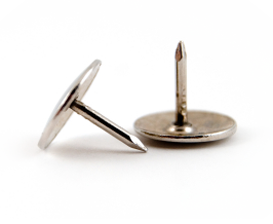
\includegraphics[scale=.5]{Thumbtacks}
\end{multicols}
\end{frame}

\end{document}
